\documentclass{article}
\usepackage[utf8]{inputenc}
\usepackage{graphicx}
\usepackage{hyperref}
\usepackage{titling}
\usepackage{array}
\usepackage{enumitem}
\usepackage{listings}
\usepackage{xcolor}
\usepackage{geometry}
\usepackage{amsmath}
\usepackage{amssymb}
\usepackage{titlesec}
\usepackage{pgfgantt}

% Float management
\usepackage{float}        % Allows [H] specifier
\usepackage{placeins}     % For \FloatBarrier
\usepackage{tabularx}     % Auto-wrap columns
\usepackage{adjustbox}    % For scaling large content (flowcharts, etc.)

% --- TikZ and PGF for flowcharts ---
\usepackage{tikz}
\usetikzlibrary{shapes.geometric, arrows}

\geometry{a4paper, margin=1in}

\setcounter{secnumdepth}{4}
\setcounter{tocdepth}{4} 

\titleformat{\paragraph}
{\normalfont\normalsize\bfseries}{\theparagraph}{1em}{}
\titlespacing*{\paragraph}
{0pt}{3.25ex plus 1ex minus .2ex}{1.5ex plus .2ex}

\definecolor{codegreen}{rgb}{0,0.6,0}
\definecolor{codegray}{rgb}{0.5,0.5,0.5}
\definecolor{codepurple}{rgb}{0.58,0,0.82}
\definecolor{backcolour}{rgb}{0.95,0.95,0.92}

% Custom lst style
\lstdefinestyle{mystyle}{
    backgroundcolor=\color{backcolour},
    commentstyle=\color{codegreen},
    keywordstyle=\color{magenta},
    numberstyle=\tiny\color{codegray},
    stringstyle=\color{codepurple},
    basicstyle=\ttfamily\footnotesize,
    breakatwhitespace=false,
    breaklines=true,
    captionpos=b,
    keepspaces=true,
    numbers=left,
    numbersep=5pt,
    showspaces=false,
    showstringspaces=false,
    showtabs=false,
    tabsize=2
}
\lstset{style=mystyle}

% TikZ flowchart styles
\tikzstyle{startstop} = [rectangle, rounded corners, minimum width=2.5cm, minimum height=0.8cm, text centered, draw=black, fill=gray!20]
\tikzstyle{io} = [trapezium, trapezium left angle=70, trapezium right angle=110, minimum width=2.8cm, minimum height=0.8cm, text centered, draw=black, fill=blue!20]
\tikzstyle{process} = [rectangle, minimum width=2.8cm, minimum height=0.8cm, text centered, draw=black, fill=orange!20]
\tikzstyle{decision} = [diamond, aspect=2, text centered, draw=black, fill=green!20]
\tikzstyle{arrow} = [thick,->,>=stealth]

\title{Clash Royale Online Implementation}
\author{Paul Hodges}
\date{\today}

\begin{document}

\begin{titlepage}
    \centering
    \vspace*{4cm}
    {\Huge \textbf{Clash Royale} \par}
    \vspace{2cm}
    {\Large by \par}
    \vspace{1cm}
    {\Large Paul Hodges \par}
    \vspace{3cm}
    {\Large \today \par}
    \vspace*{4cm}
\end{titlepage}

\tableofcontents
\newpage

\section{Development Schedule}

\begin{ganttchart}[
    hgrid,
    vgrid={*{4}{gray, dotted}, *1{black, dashed}},
    bar label node/.append style={align=left},
    bar/.append style={fill=blue!40},
    group/.append style={fill=blue!20},
    milestone/.append style={fill=red, inner sep=2pt},
    title label font=\bfseries\footnotesize,
    bar label font=\footnotesize,
    y unit chart=0.5cm,
    x unit=11pt,
    canvas/.style={draw=none, fill=none},
    today=7,
    today rule/.style={
      draw=red,
      dash pattern=on 3.5pt off 4.5pt,
      line width=1.5pt
    },
    today label={Today},
    today label font=\small\bfseries,
    today label node/.append style={below=7pt},
    progress label node/.append style={below right=10pt},
    link/.style={->, thick, rounded corners=2pt},
    title/.style={draw=none, fill=white},
    title label node/.append style={below=0pt},
    title height=0.75,
    bar height=0.6,
    milestone height=0.6,
    group top shift=0.5,
    group height=0.2
]{1}{28}
% Title row with weeks
\gantttitle{Week 1}{7} \gantttitle{Week 2}{7} \gantttitle{Week 3}{7} \gantttitle{Week 4}{7} \\
% Main project phases with grouping - with no connections
\ganttgroup[group/.append style={fill=blue!20}]{1. Core Engine \& Network}{1}{7} \\
    \ganttbar[bar/.append style={fill=blue!50}]{Engine Setup}{1}{3} \\
    \ganttbar[bar/.append style={fill=blue!50}]{Network Setup}{4}{7} \\
    \ganttmilestone[milestone/.append style={fill=red}]{Core Platform Complete}{7} \\
\ganttgroup[group/.append style={fill=green!20}]{2. Gameplay Mechanics}{8}{14} \\
    \ganttbar[bar/.append style={fill=green!50}]{ECS + Cards Implementation}{8}{10} \\
    \ganttbar[bar/.append style={fill=green!50}]{Gameplay Logic}{11}{14} \\
    \ganttmilestone[milestone/.append style={fill=red}]{Gameplay Prototype Ready}{14} \\
\ganttgroup[group/.append style={fill=orange!20}]{3. Progression \& Rewards}{15}{21} \\
    \ganttbar[bar/.append style={fill=orange!50}]{Progression System}{15}{18} \\
    \ganttbar[bar/.append style={fill=orange!50}]{Database + Security}{19}{21} \\
    \ganttmilestone[milestone/.append style={fill=red}]{Systems Integration Complete}{21} \\
\ganttgroup[group/.append style={fill=purple!20}]{4. Testing \& Refinement}{22}{28} \\
    \ganttbar[bar/.append style={fill=purple!50}]{Core Testing}{22}{23} \\
    \ganttbar[bar/.append style={fill=purple!50}]{Gameplay Testing}{24}{26} \\
    \ganttbar[bar/.append style={fill=purple!50}]{Final Testing \& Bugfixes}{27}{28} \\
    \ganttmilestone[milestone/.append style={fill=red}]{Release Candidate Ready}{28} \\

\end{ganttchart}

\section{Problem Outline}

The purpose of this project is to develop a simplified but functional online version of Clash Royale using Python. This real-time strategy game implementation will focus on core gameplay mechanics and network functionality, demonstrating practical software development skills in a gaming context.

\noindent The game will allow players to:
\begin{itemize}
    \item Engage in real-time, online strategic battles against other players
    \item Build and customize card decks from their collection
    \item Progress through a skill-based arena system
    \item Earn rewards through a chest system to expand their card collection
    \item Experience the core strategic elements that make Clash Royale engaging
\end{itemize}

\noindent This implementation serves as both an educational tool for understanding game development principles and a demonstration of networking, database management, and software architecture skills in a cohesive application.

\section{Problem Description}

\subsection{Game Overview}
Clash Royale is a real-time strategy game where players deploy cards representing troops, spells, and buildings onto a battlefield to defeat their opponent. The game combines elements of collectible card games, tower defense, and multiplayer online battle arenas (MOBAs) into a unique gaming experience.

\subsection{Game Objectives}
The primary objective is to destroy more of the opponent's towers than they destroy of yours within the allotted battle time (typically 3 minutes, with a 2 minute overtime if tied). The game features:
\begin{itemize}
    \item Three towers per player: two Princess Towers and one King Tower
    \item Destroying a Princess Tower grants one crown
    \item Destroying the King Tower grants three crowns and ends the match immediately
    \item The player with more crowns at the end of the time limit wins
\end{itemize}

\subsection{Core Game Rules}
\begin{itemize}
    \item Each player begins with four cards from their eight-card deck
    \item Cards are deployed using elixir, a regenerating resource
    \item Elixir regenerates at a rate of 1 unit every 2.8 seconds (doubles in the first minute of overtime and then triples in the second minute)
    \item Maximum elixir capacity is 10 units
    \item Card costs range from 1 to 8 elixir
    \item After playing a card, it's replaced by another from the player's deck
    \item Cards can only be deployed on the player's side of the arena (with exceptions for spells and certain cards)
    \item Units automatically move toward and attack enemy units and towers based on their targeting preferences
\end{itemize}

\subsection{Gameplay Flow}
\begin{enumerate}
    \item Players join a match through the matchmaking system
    \item Both players start with the same amount of elixir
    \item Players strategically deploy cards to attack opponent towers while defending their own
    \item Units and buildings have specific health, damage, speed, and targeting parameters
    \item Spells cause immediate effects (damage, slow, etc.) in their area of effect
    \item Destroyed units are removed from the battlefield
    \item The battle continues until a King Tower falls or time expires
\end{enumerate}

\subsection{Scoring System}
\begin{itemize}
    \item Destroying a Princess Tower: 1 crown
    \item Destroying the King Tower: 3 crowns (automatic victory)
    \item Most crowns at time expiration: Victory
    \item Equal crowns at time expiration: Draw
    \item Victory awards trophies that contribute to arena progression
    \item Defeat results in trophy loss
\end{itemize}

\subsection{Winner Determination}
\begin{itemize}
    \item The player who destroys the opponent's King Tower instantly wins
    \item If no King Tower is destroyed within the time limit, the player with more crowns wins
    \item If both players have the same number of crowns when time expires, the match enters overtime
    \item In overtime, the first player to gain a crown advantage wins
    \item If neither player gains an advantage during overtime, the match ends in a draw
\end{itemize}

\subsection{Advanced Game Mechanics and Strategies}
\begin{itemize}
    \item \textbf{Elixir Management:} Efficient use of elixir is critical; overspending creates vulnerability
    \item \textbf{Counter Deployment:} Specific cards counter others effectively (e.g., air units counter ground-only attackers)
    \item \textbf{Card Synergies:} Certain combinations of cards create powerful offensive or defensive capabilities
    \item \textbf{Lane Pressure:} Applying pressure in one lane to force defensive card usage, then attacking the other
    \item \textbf{Elixir Counting:} Tracking opponent's elixir to identify advantageous attack opportunities
    \item \textbf{Card Cycle Management:} Cycling through cards quickly to reach key cards in your deck
    \item \textbf{Tower Trading:} Strategic sacrifice of a tower to gain elixir advantage for a stronger counter-push
    \item \textbf{Spell Value:} Using spells to eliminate multiple units simultaneously for positive elixir trades
    \item \textbf{Unit Placement:} Precise placement affects unit interactions and pathing
    \item \textbf{Timing:} Deploying cards at optimal moments to maximize their effectiveness
\end{itemize}

\section{Requirements}

\subsection{Functional Requirements}

\begin{enumerate}
    \item \textbf{FR1: Server-Client Architecture}
    \begin{itemize}
        \item The system shall implement a client-server model supporting real-time multiplayer
        \item The server shall handle game state synchronization across clients
        \item The server shall manage concurrent games with minimal latency
        \item The system shall handle connection drops and reconnections gracefully
    \end{itemize}

    \item \textbf{FR2: Card Management System}
    \begin{itemize}
        \item Players shall be able to view their card collection
        \item Players shall be able to build decks with exactly 8 cards
        \item The system shall validate deck composition rules
        \item The system shall implement card rarity and level mechanics
        \item Players shall be able to upgrade cards when meeting requirements
    \end{itemize}

    \item \textbf{FR3: Real-time Battle Simulation}
    \begin{itemize}
        \item The system shall manage battles in real-time
        \item The system shall implement elixir generation mechanics
        \item The system shall handle unit deployment, movement, and targeting
        \item The system shall calculate damage, health, and tower destruction
        \item The system shall implement the 3-minute standard time and overtime rules
    \end{itemize}

    \item \textbf{FR4: Progression System}
    \begin{itemize}
        \item The system shall track player trophies
        \item The system shall implement arena progression based on trophy count
        \item The system shall match players based on similar trophy counts
        \item Different arenas shall unlock different cards
    \end{itemize}

    \item \textbf{FR5: Reward System}
    \begin{itemize}
        \item The system shall reward players with chests after victories
        \item Chests shall contain cards and gold based on arena level
        \item The system shall implement various chest types with different rewards
        \item The system shall track chest unlocking timers
    \end{itemize}

    \item \textbf{FR6: Clan System}
    \begin{itemize}
        \item Players shall be able to create and join clans
        \item Clans shall support basic member management
        \item The system shall implement a clan chat feature
        \item The system shall display clan member activity
    \end{itemize}

    \item \textbf{FR7: User Authentication}
    \begin{itemize}
        \item The system shall securely authenticate users
        \item The system shall protect user credentials
        \item The system shall manage login sessions with tokens
        \item The system shall enforce password security requirements
    \end{itemize}

    \item \textbf{FR8: Database Integration}
    \begin{itemize}
        \item The system shall persist all player data
        \item The system shall record battle history
        \item The system shall implement transaction safety for critical operations
        \item The system shall backup data regularly
    \end{itemize}
\end{enumerate}

\subsection{Non-Functional Requirements}

\begin{enumerate}
    \item \textbf{NFR1: Performance}
    \begin{itemize}
        \item The system shall handle at least 100 concurrent connections
        \item Battle simulations shall update at least 10 times per second
        \item Server response time shall not exceed 200ms under normal load
        \item Client frame rate shall maintain at least 30 FPS on target devices
    \end{itemize}

    \item \textbf{NFR2: Reliability}
    \begin{itemize}
        \item The system shall have 99\% uptime
        \item The system shall recover from crashes without data loss
        \item The system shall handle network instability gracefully
        \item The system shall implement data integrity checks
    \end{itemize}

    \item \textbf{NFR3: Scalability}
    \begin{itemize}
        \item The architecture shall support horizontal scaling
        \item The database shall handle growing player data efficiently
        \item The matchmaking algorithm shall scale with player population
    \end{itemize}

    \item \textbf{NFR4: Maintainability}
    \begin{itemize}
        \item The code shall follow PEP 8 style guidelines
        \item The system shall use modular design patterns
        \item The codebase shall include comprehensive documentation
        \item The system shall implement logging for debugging
    \end{itemize}

    \item \textbf{NFR5: Security}
    \begin{itemize}
        \item User passwords shall be stored using strong hashing
        \item Communication shall be encrypted
        \item The system shall protect against common attack vectors
        \item The system shall validate all client input
    \end{itemize}
\end{enumerate}

\section{Design}

\subsection{Core System Design}

The game will be built using a custom Entity Component System (ECS) engine and a custom network implementation. The visual style will be 2D with a simulated 3D look achieved through layered sprites and shadow rendering.

\subsubsection{Engine}

The engine is written in Python, based on the design off of one of my previous Rust engines, "Oxidized." Key features include:

\paragraph{ECS Architecture}

The Entity Component System (ECS) architecture separates data (components) from logic (systems). Entities are simple IDs, and components are data containers (e.g., Position, Velocity, Sprite). Systems operate on entities that have the required components. This design promotes data-oriented programming, improving cache efficiency and making the code more modular and maintainable. In this Python implementation, I leverage dictionaries and lists to store and manage entities, components, and systems. For example, a "MovementSystem" would iterate through entities with "Position" and "Velocity" components, updating their positions based on their velocities. This decoupling of data and logic allows for flexible entity composition and avoids the complexities of traditional inheritance-based object-oriented programming.

\paragraph{2D/3D Cameras}
The engine will support both orthographic and perspective cameras. Orthographic cameras provide a parallel projection, useful for classic 2D views where depth isn't emphasized. Perspective cameras simulate real-world vision, where objects appear smaller as they recede into the distance. This is crucial for creating the simulated 3D look. The camera implementation will likely involve a transformation matrix that converts world coordinates to screen coordinates. For perspective cameras, this matrix will include a perspective projection component, while orthographic cameras will use a simple scaling and translation matrix. I have functions to easily switch between camera types, and to adjust the field of view of the perspective camera.

\paragraph{GameObjects and Components}
GameObjects serve as containers for components. By assigning different combinations of components to a GameObject, I can create a wide variety of entities with unique behaviors. For example, a "Player" GameObject might have "Position," "Velocity," "Sprite," "Input," and "Health" components. A "Tree" GameObject might have "Position" and "Sprite" components. This modularity allows for easy creation and modification of game entities without modifying core engine code. The component data will be stored in data structures that are easily accessible by the systems.

\paragraph{Layered Sprite Rendering}
To create the illusion of depth in a 2D environment, I will use layered sprites. Sprites representing objects closer to the "camera" will be rendered on top of sprites representing objects further away. I will implement a sorting mechanism based on the Y-coordinate (or a custom depth value) of the entities to determine the rendering order. This will allow for overlapping sprites to create a sense of depth. Furthermore, I will have the capability to assign a layer number to each sprite, allowing for more manual control over the draw order, and enabling the creation of backgrounds, midgrounds, and foregrounds.

\paragraph{Rendering}
The rendering for the python engine are not done using conventional methods like "pygame". I use a custom library that i created myself which uses SDL2 to draw to the screen and provides more complex methods for other things like textures, images and keyboard input. I create the python bindings (for the cpython module) using pybin11. The library is compiled, the binds are compiled and then the library is linked with the binds to produce a cpython library. The stub file for the LSP is then generated using stubgen, which is shipped with python.

\subsubsection{Network}

The network uses custom socket communication with binary data transmission:

\paragraph{Custom Binary Protocol}
Instead of relying on human-readable text-based protocols, I use a custom binary protocol. This protocol will define the structure of packets sent between the client and server, specifying the types and sizes of data fields. Binary protocols are more compact and efficient, reducing network overhead and latency. I will use python's struct module to pack and unpack data into binary format. I will define packet types, and each packet type will have a defined data structure.

\paragraph{Client-Server Architecture}
I will implement a client-server architecture, where the server acts as the authoritative source of game state. Clients send input to the server, and the server processes the input, updates the game state, and sends updates back to the clients. This architecture helps prevent cheating and ensures consistency across all clients. The server will maintain the master copy of the game world, and the clients will maintain local copies that are kept in sync with the server.

\paragraph{Asynchronous Sockets}
To avoid blocking the main game loop, I will use asynchronous sockets. Asynchronous sockets allow the game to continue running while waiting for network data. I will use python's asyncio library or similar, to handle the asynchronous network operations. This will prevent the game from freezing or becoming unresponsive during network communication.

\paragraph{Packet Listener and Broadcaster}
The server will have a packet listener to receive incoming packets from clients and a packet broadcaster to send packets to all connected clients. The listener will parse incoming packets and dispatch them to the appropriate game logic. The broadcaster will efficiently distribute game state updates to all clients, minimizing network traffic. I will implement packet queuing and throttling to prevent network congestion. The broadcaster will only send data that has changed, to reduce the amount of data sent.

\subsubsection{2D with 3D Illusion}

The 3D look is achieved through:

\paragraph{Layered Sprites}
As mentioned earlier, layered sprites are crucial for creating the illusion of depth. By rendering sprites in a specific order based on their perceived depth, I can simulate the effect of objects being in front of or behind each other. This will involve sorting sprites by their Y-coordinate or a custom depth value before rendering. I will use a depth buffer, or an equivalent sort algorithm, to ensure that sprites are drawn in the correct order.

\paragraph{Shadow Rendering}
Adding shadows to objects can significantly enhance depth perception. I will implement shadow rendering by projecting a simplified silhouette of each object onto the ground. The darkness and length of the shadow will vary based on the object's height and the light source's position. This will give objects a sense of grounding and add visual depth to the scene. I will use sprite masks to create the shadow silhouettes.

\paragraph{Perspective Scaling}
To further enhance the 3D illusion, I will implement perspective scaling. Objects farther away from the "camera" will appear smaller, while objects closer will appear larger. This will be achieved by adjusting the sprite's scale based on its distance from the camera. I will use a perspective projection matrix to calculate the scale factor. This will be done in conjunction with the Layered Sprite rendering, to create a believable 3D effect.

\subsection{Algorithm Design}

Below are the core algorithms for the main game systems.

%---------------------------------------------
% MAIN SERVER LOOP
%---------------------------------------------
\subsubsection{Main Server Loop}
\begin{lstlisting}[language=Python, caption=Main Server Loop]
FUNCTION RunServer():
    INITIALIZE server
    INITIALIZE player_pool = []
    INITIALIZE active_games = []

    WHILE server_running:
        FOR each incoming_connection:
            IF is_new_connection THEN
                player = CreatePlayer(connection)
                player_pool.APPEND(player)
                SEND_WELCOME_MESSAGE(connection)
            ELSE IF is_matchmaking_request THEN
                player = GetPlayerFromConnection(connection)
                MatchmakingQueue.ADD(player)
            ELSE IF is_game_action THEN
                game = GetGameFromPlayer(connection)
                ProcessGameAction(game, connection, action)
            END IF
        END FOR

        # Matchmaking
        WHILE MatchmakingQueue.COUNT >= 2:
            player1 = MatchmakingQueue.GET_NEXT()
            player2 = MatchmakingQueue.FIND_OPPONENT(player1)
            IF player2 != NULL THEN
                game = CreateGame(player1, player2)
                active_games.APPEND(game)
                MatchmakingQueue.REMOVE(player2)
            ELSE
                MatchmakingQueue.RETURN(player1)
                BREAK
            END IF
        END WHILE

        # Update all active games
        FOR each game IN active_games:
            UpdateGame(game)
            IF game.is_finished THEN
                ProcessGameResults(game)
                active_games.REMOVE(game)
            END IF
        END FOR
    END WHILE
END FUNCTION
\end{lstlisting}

\FloatBarrier

%---------------------------------------------
% CARD DEPLOYMENT
%---------------------------------------------
\subsubsection{Card Deployment Process}
\begin{lstlisting}[language=Python, caption=Card Deployment]
FUNCTION ProcessCardDeployment(game, player, card_id, position_x, position_y):
    # Validate the deployment
    IF NOT IsValidDeployPosition(game, player, position_x, position_y) THEN
        SEND_ERROR(player, "Invalid deployment position")
        RETURN False
    END IF

    # Get the card from player's hand
    card = player.GetCardFromHand(card_id)
    IF card == NULL THEN
        SEND_ERROR(player, "Card not in hand")
        RETURN False
    END IF

    # Check elixir cost
    IF player.current_elixir < card.elixir_cost THEN
        SEND_ERROR(player, "Insufficient elixir")
        RETURN False
    END IF

    # Deploy the card
    player.current_elixir = player.current_elixir - card.elixir_cost
    player.RemoveCardFromHand(card_id)
    player.AddNextCardToHand()

    # Create the unit/spell/building on the field
    IF card.type == "TROOP" THEN
        unit = CreateTroop(card, position_x, position_y, player.side)
        game.AddUnit(unit)
    ELSE IF card.type == "SPELL" THEN
        ApplySpellEffect(game, card, position_x, position_y, player.side)
    ELSE IF card.type == "BUILDING" THEN
        building = CreateBuilding(card, position_x, position_y, player.side)
        game.AddBuilding(building)
    END IF

    # Notify both players
    BROADCAST_DEPLOYMENT(game, player.id, card_id, position_x, position_y)

    RETURN True
END FUNCTION
\end{lstlisting}

\FloatBarrier

%---------------------------------------------
% BATTLE UPDATE LOGIC
%---------------------------------------------
\subsubsection{Battle Update Logic}
\begin{lstlisting}[language=Python, caption=Battle Update Logic]
FUNCTION UpdateGame(game):
    # Update game time
    game.current_time = game.current_time + TICK_RATE

    # Check for game end conditions
    IF game.current_time >= game.max_time AND NOT game.in_overtime THEN
        IF game.player1.crowns == game.player2.crowns THEN
            game.in_overtime = True
            game.overtime_end = game.current_time + OVERTIME_DURATION
            BROADCAST_OVERTIME_START(game)
        ELSE
            game.is_finished = True
            RETURN
        END IF
    END IF

    IF game.in_overtime AND game.current_time >= game.overtime_end THEN
        game.is_finished = True
        RETURN
    END IF

    # Regenerate elixir
    regeneration_amount = CALCULATE_ELIXIR_REGEN(game)
    game.player1.current_elixir = MIN(game.player1.current_elixir + regeneration_amount, MAX_ELIXIR)
    game.player2.current_elixir = MIN(game.player2.current_elixir + regeneration_amount, MAX_ELIXIR)

    # Update all units
    FOR each unit IN game.units:
        IF unit.health <= 0 THEN
            game.RemoveUnit(unit)
            CONTINUE

        # Find target
        IF unit.current_target == NULL OR unit.current_target.health <= 0 THEN
            unit.current_target = FindTarget(game, unit)
        END IF

        # Move/attack
        IF unit.current_target != NULL THEN
            IF IsInRange(unit, unit.current_target) THEN
                PerformAttack(unit, unit.current_target)
            ELSE
                MoveTowards(unit, unit.current_target)
            END IF
        END IF
    END FOR

    # Update buildings
    FOR each building IN game.buildings:
        IF building.health <= 0 OR building.lifetime <= 0 THEN
            game.RemoveBuilding(building)
            CONTINUE

        building.lifetime = building.lifetime - TICK_RATE

        IF building.can_attack THEN
            IF building.current_target == NULL OR building.current_target.health <= 0 THEN
                building.current_target = FindTarget(game, building)
            END IF
            IF building.current_target != NULL AND IsInRange(building, building.current_target) THEN
                PerformAttack(building, building.current_target)
            END IF
        END IF
    END FOR

    # Check towers
    CheckTowerStatus(game)

    # Broadcast state
    BROADCAST_GAME_STATE(game)
END FUNCTION
\end{lstlisting}

\FloatBarrier

%---------------------------------------------
% TARGET SELECTION ALGORITHM
%---------------------------------------------
\subsubsection{Target Selection Algorithm}
\begin{lstlisting}[language=Python, caption=Target Finding]
FUNCTION FindTarget(game, attacker):
    closest_target = NULL
    min_distance = INFINITY

    # Determine potential targets
    potential_targets = []
    IF attacker.attacks_ground AND attacker.attacks_air THEN
        potential_targets = game.GetAllUnitsAndBuildings(GetOpponentSide(attacker.side))
    ELSE IF attacker.attacks_ground THEN
        potential_targets = game.GetGroundUnitsAndBuildings(GetOpponentSide(attacker.side))
    ELSE IF attacker.attacks_air THEN
        potential_targets = game.GetAirUnits(GetOpponentSide(attacker.side))
    END IF

    # Add towers
    towers = game.GetTowers(GetOpponentSide(attacker.side))
    potential_targets.EXTEND(towers)

    # Targeting preference
    IF attacker.targeting_preference == "BUILDINGS":
        buildings = [t FOR t IN potential_targets IF t.type == "BUILDING" OR t.type == "TOWER"]
        IF buildings.LENGTH > 0:
            potential_targets = buildings

    # Find closest
    FOR each target IN potential_targets:
        distance = CalculateDistance(attacker.position, target.position)
        IF distance < min_distance:
            min_distance = distance
            closest_target = target

    RETURN closest_target
END FUNCTION
\end{lstlisting}

\FloatBarrier

%---------------------------------------------
% CHEST REWARD SYSTEM
%---------------------------------------------
\subsubsection{Chest Reward System}
\begin{lstlisting}[language=Python, caption=Chest Generation]
FUNCTION GenerateChestForPlayer(player, chest_type):
    # Create a new chest
    chest = CreateChest(chest_type)

    # Set unlock time
    IF chest_type == "SILVER":
        chest.unlock_time = 3 * HOURS
    ELSE IF chest_type == "GOLD":
        chest.unlock_time = 8 * HOURS
    ELSE IF chest_type == "MAGICAL":
        chest.unlock_time = 12 * HOURS
    ELSE IF chest_type == "GIANT":
        chest.unlock_time = 16 * HOURS

    # Gold reward
    chest.gold = CALCULATE_GOLD_REWARD(player.arena, chest_type)

    # Card counts
    common_count, rare_count, epic_count, legendary_count = CALCULATE_CARD_COUNTS(player.arena, chest_type)

    # Generate cards
    available_cards = GetAvailableCardsForArena(player.arena)

    FOR i = 1 TO common_count:
        card = SelectRandomCard(available_cards, "COMMON")
        chest.AddCard(card)

    FOR i = 1 TO rare_count:
        card = SelectRandomCard(available_cards, "RARE")
        chest.AddCard(card)

    FOR i = 1 TO epic_count:
        card = SelectRandomCard(available_cards, "EPIC")
        chest.AddCard(card)

    FOR i = 1 TO legendary_count:
        card = SelectRandomCard(available_cards, "LEGENDARY")
        chest.AddCard(card)

    # Add to player's inventory
    player.AddChest(chest)

    # Notify
    SEND_CHEST_RECEIVED(player, chest)
    RETURN chest
END FUNCTION
\end{lstlisting}

\FloatBarrier

%---------------------------------------------
% FLOWCHARTS
%---------------------------------------------
\subsection{Algorithm Flowcharts}

\subsubsection{Main Server Loop Flowchart}
\begin{figure}[H]
\centering
% Scale to 80% of page height to ensure it fits
\adjustbox{max height=0.8\textheight}{%
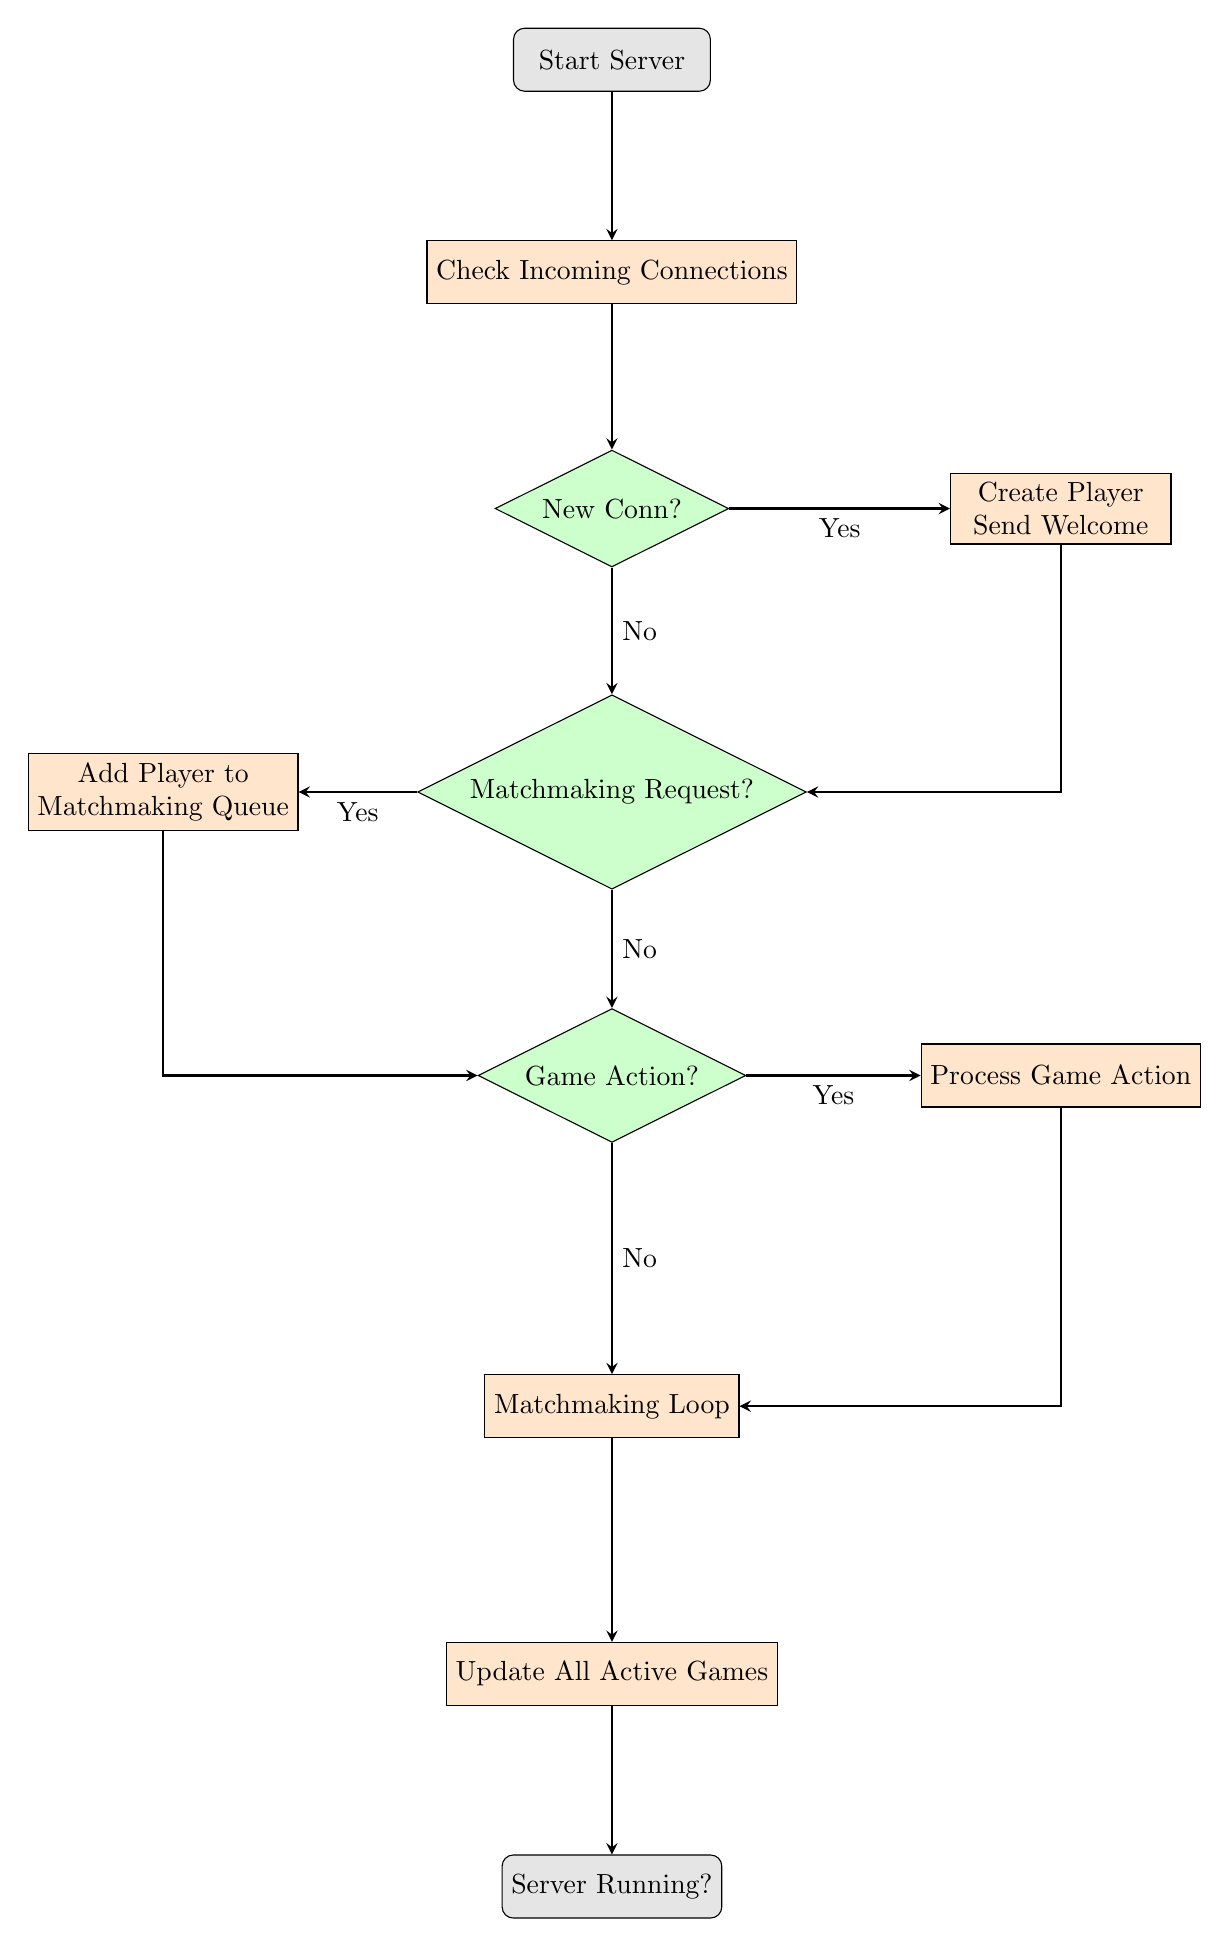
\begin{tikzpicture}[node distance=2.2cm]
\node (start) [startstop] {Start Server};
\node (conn) [process, below of=start, yshift=-0.5cm] {Check Incoming Connections};
\node (decNew) [decision, below of=conn, yshift=-0.8cm] {New Conn?};
\node (createP) [process, right of=decNew, xshift=3.5cm, align=center] {Create Player \\ Send Welcome};
\node (decMatch) [decision, below of=decNew, yshift=-1.4cm] {Matchmaking Request?};
\node (addMatch) [process, left of=decMatch, xshift=-3.5cm, align=center] {Add Player to \\ Matchmaking Queue};
\node (decGameA) [decision, below of=decMatch, yshift=-1.4cm] {Game Action?};
\node (procGameA) [process, right of=decGameA, xshift=3.5cm] {Process Game Action};
\node (matchmake) [process, below of=decGameA, yshift=-2.0cm] {Matchmaking Loop};
\node (updateGames) [process, below of=matchmake, yshift=-1.2cm] {Update All Active Games};
\node (end) [startstop, below of=updateGames, yshift=-0.5cm] {Server Running?};

\draw [arrow] (start) -- (conn);
\draw [arrow] (conn) -- (decNew);
\draw [arrow] (decNew) -- node[anchor=north] {Yes} (createP);
\draw [arrow] (decNew) -- node[anchor=west] {No} (decMatch);
\draw [arrow] (createP) |- (decMatch);
\draw [arrow] (decMatch) -- node[anchor=north] {Yes} (addMatch);
\draw [arrow] (decMatch) -- node[anchor=west] {No} (decGameA);
\draw [arrow] (addMatch) |- (decGameA);
\draw [arrow] (decGameA) -- node[anchor=north] {Yes} (procGameA);
\draw [arrow] (decGameA) -- node[anchor=west] {No} (matchmake);
\draw [arrow] (procGameA) |- (matchmake);
\draw [arrow] (matchmake) -- (updateGames);
\draw [arrow] (updateGames) -- (end);
% \draw [arrow] (end) -- ++(0,-1.0) node[anchor=north] {Yes} -| (conn);
\end{tikzpicture}%
} % end adjustbox
\caption{Main Server Loop Flowchart}
\end{figure}

\FloatBarrier

\subsubsection{Card Deployment Process Flowchart}
\begin{figure}[H]
\centering
\adjustbox{max height=0.8\textheight}{%
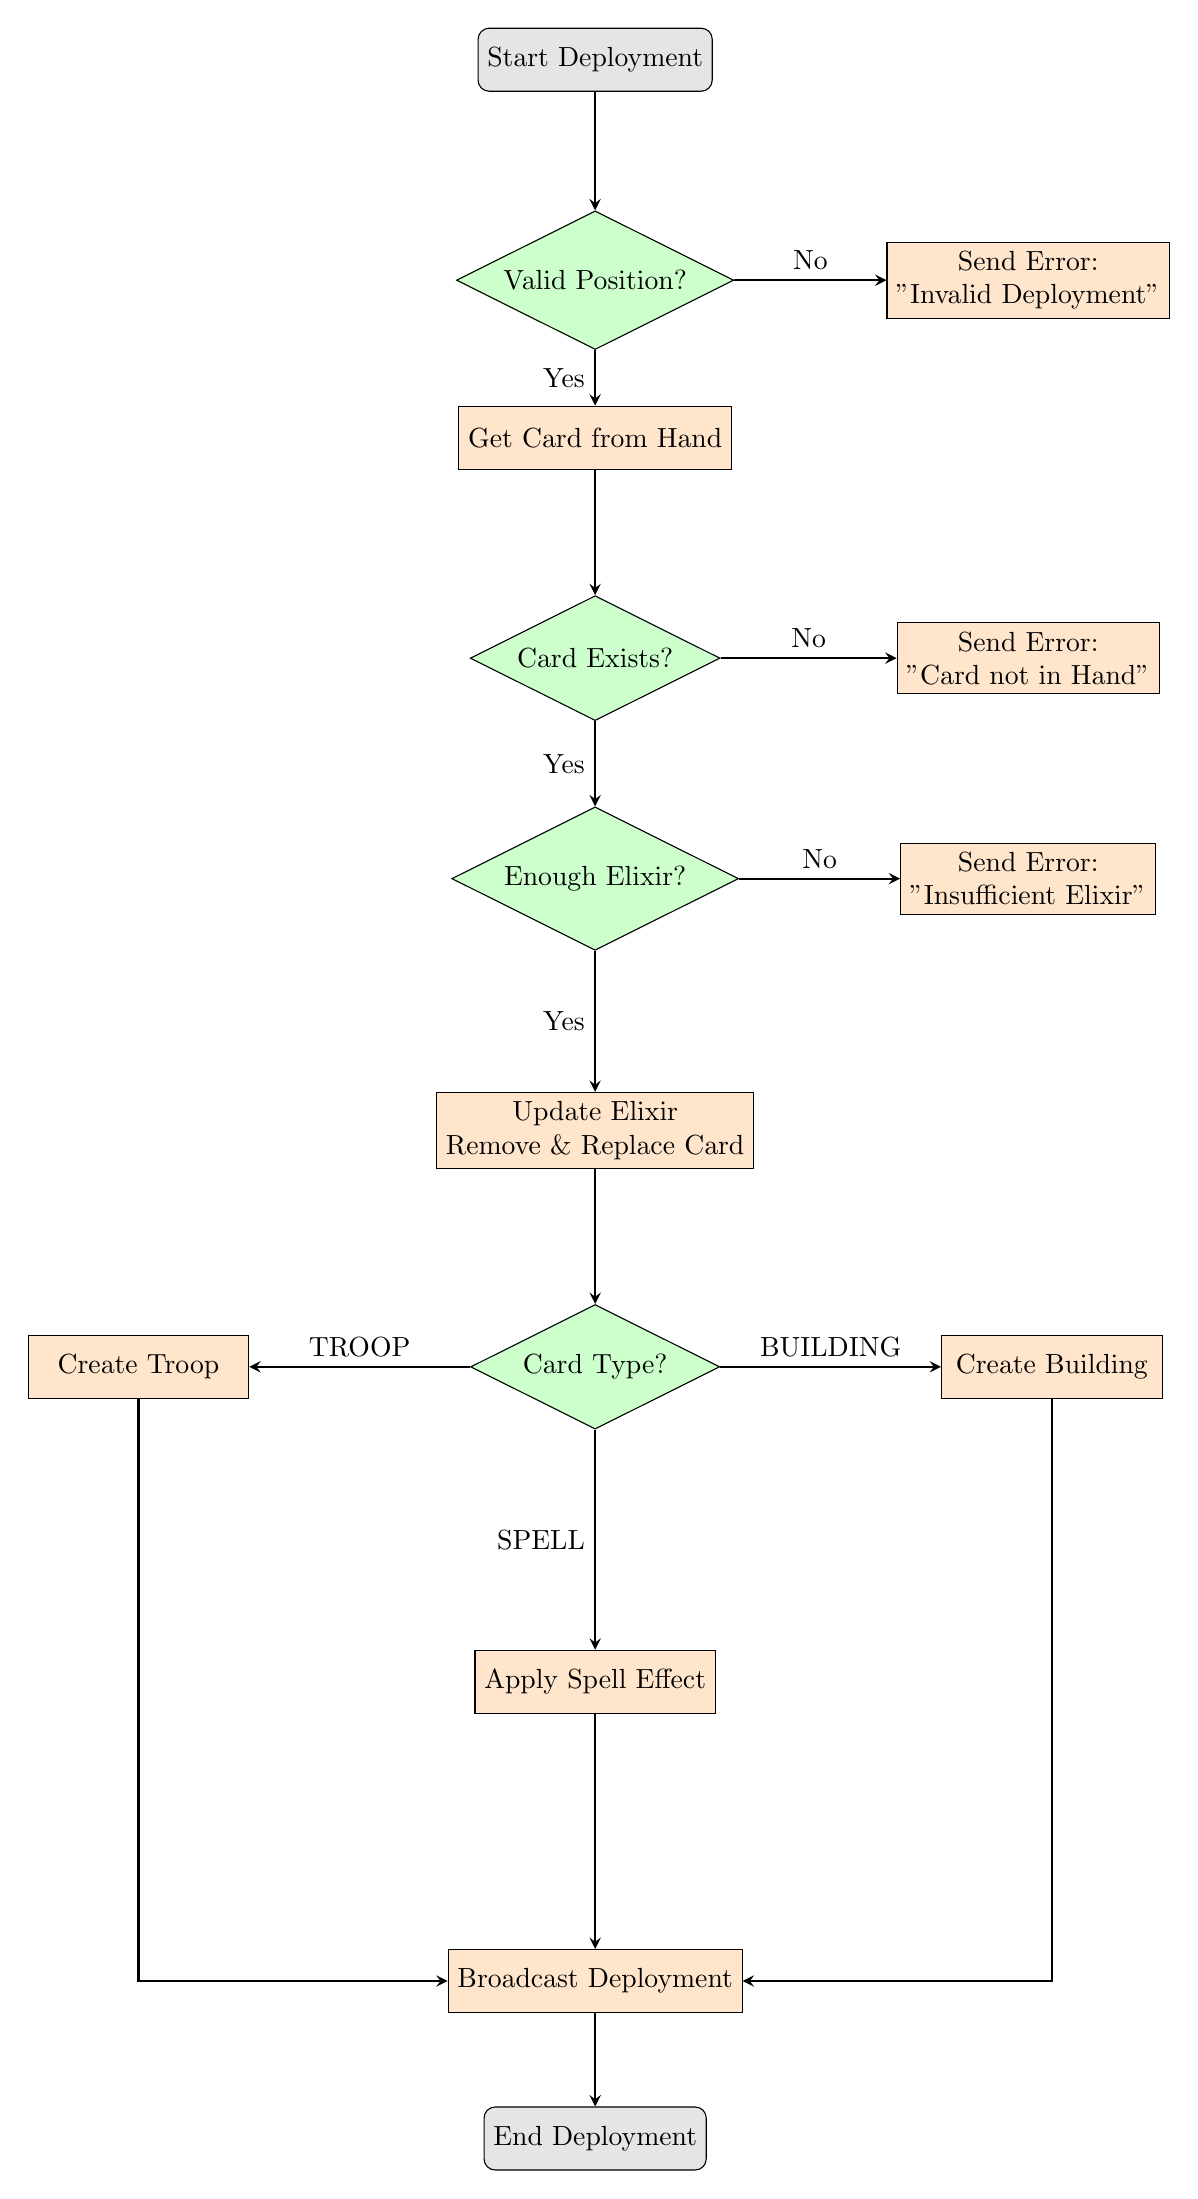
\begin{tikzpicture}[node distance=2cm]
\node (start) [startstop] {Start Deployment};
\node (checkPos) [decision, below of=start, yshift=-0.8cm] {Valid Position?};
\node (errorPos) [process, right of=checkPos, xshift=3.5cm, align=center] {Send Error: \\
"Invalid Deployment"};
\node (getCard) [process, below of=checkPos] {Get Card from Hand};
\node (cardNull) [decision, below of=getCard, yshift=-0.8cm] {Card Exists?};
\node (errorCard) [process, right of=cardNull, xshift=3.5cm, align=center] {Send Error: \\
"Card not in Hand"};
\node (checkElixir) [decision, below of=cardNull, yshift=-0.8cm] {Enough Elixir?};
\node (errorElixir) [process, right of=checkElixir, xshift=3.5cm, align=center] {Send Error: \\
"Insufficient Elixir"};
\node (deploy) [process, below of=checkElixir, yshift=-1.2cm,align=center] {Update Elixir \\
Remove \& Replace Card};
\node (typeCheck) [decision, below of=deploy, yshift=-1.0cm] {Card Type?};
\node (troop) [process, left of=typeCheck, xshift=-3.8cm] {Create Troop};
\node (spell) [process, below of=typeCheck, yshift=-2.0cm] {Apply Spell Effect};
\node (building) [process, right of=typeCheck, xshift=3.8cm] {Create Building};
\node (broadcast) [process, below of=spell, yshift=-1.8cm] {Broadcast Deployment};
\node (end) [startstop, below of=broadcast] {End Deployment};

\draw [arrow] (start) -- (checkPos);
\draw [arrow] (checkPos) -- node[anchor=east] {Yes} (getCard);
\draw [arrow] (checkPos) -- node[anchor=south] {No} (errorPos);
\draw [arrow] (getCard) -- (cardNull);
\draw [arrow] (cardNull) -- node[anchor=east] {Yes} (checkElixir);
\draw [arrow] (cardNull) -- node[anchor=south] {No} (errorCard);
\draw [arrow] (checkElixir) -- node[anchor=east] {Yes} (deploy);
\draw [arrow] (checkElixir) -- node[anchor=south] {No} (errorElixir);
\draw [arrow] (deploy) -- (typeCheck);
\draw [arrow] (typeCheck) -- node[anchor=south] {TROOP} (troop);
\draw [arrow] (typeCheck) -- node[anchor=east] {SPELL} (spell);
\draw [arrow] (typeCheck) -- node[anchor=south] {BUILDING} (building);
\draw [arrow] (troop) |- (broadcast);
\draw [arrow] (spell) -- (broadcast);
\draw [arrow] (building) |- (broadcast);
\draw [arrow] (broadcast) -- (end);
\end{tikzpicture}%
}
\caption{Card Deployment Flowchart}
\end{figure}

\FloatBarrier

\subsubsection{Battle Update Logic Flowchart}
\begin{figure}[H]
\centering
\adjustbox{max height=0.8\textheight}{%
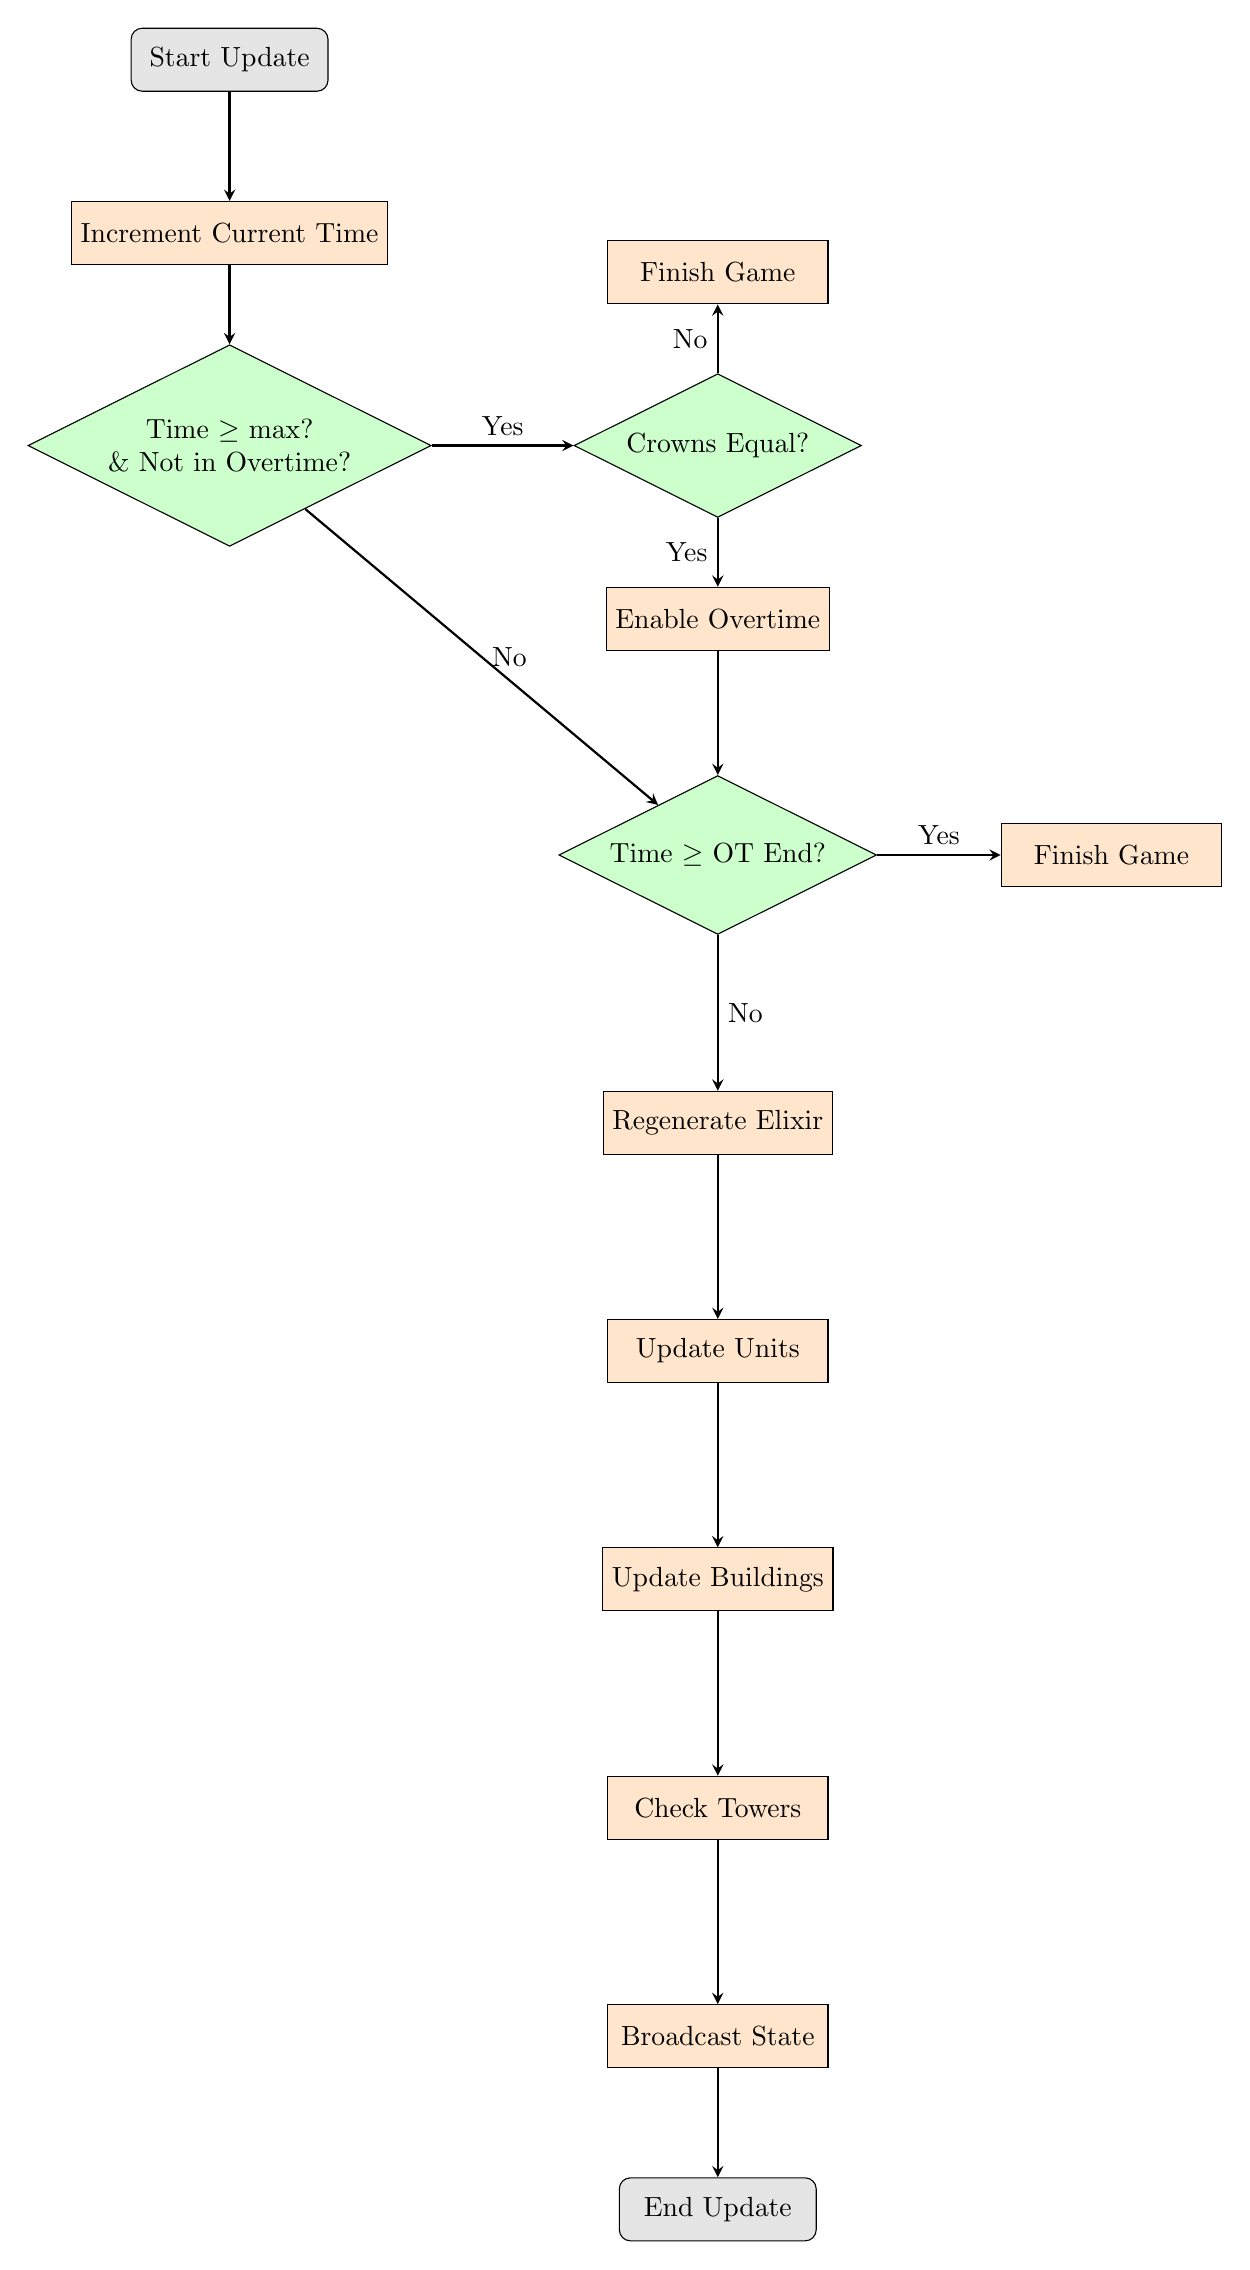
\begin{tikzpicture}[node distance=2.2cm]
\node (start) [startstop] {Start Update};
\node (timeCheck) [process, below of=start] {Increment Current Time};
\node (decOvertime) [decision, below of=timeCheck, yshift=-0.5cm,align=center] {Time $\ge$ max? \\ \& Not in Overtime?};
\node (decCrowns) [decision, right of=decOvertime, xshift=4cm] {Crowns Equal?};
\node (setOvertime) [process, below of=decCrowns] {Enable Overtime};
\node (finishGame) [process, above of=decCrowns, yshift=0.0cm] {Finish Game};
\node (otCheck) [decision, below of=setOvertime, yshift=-0.8cm] {Time $\ge$ OT End?};
\node (finishGame2) [process, right of=otCheck, xshift=2.8cm] {Finish Game};
\node (regen) [process, below of=otCheck, yshift=-1.2cm] {Regenerate Elixir};
\node (units) [process, below of=regen, yshift=-0.7cm] {Update Units};
\node (buildings) [process, below of=units, yshift=-0.7cm] {Update Buildings};
\node (checkTowers) [process, below of=buildings, yshift=-0.7cm] {Check Towers};
\node (broadcast) [process, below of=checkTowers, yshift=-0.7cm] {Broadcast State};
\node (end) [startstop, below of=broadcast] {End Update};

\draw [arrow] (start) -- (timeCheck);
\draw [arrow] (timeCheck) -- (decOvertime);
\draw [arrow] (decOvertime) -- node[anchor=south] {Yes} (decCrowns);
\draw [arrow] (decOvertime) -- node[anchor=west] {No} (otCheck);
\draw [arrow] (decCrowns) -- node[anchor=east] {Yes} (setOvertime);
\draw [arrow] (decCrowns) -- node[anchor=east] {No} (finishGame);
\draw [arrow] (setOvertime) -- (otCheck);
\draw [arrow] (otCheck) -- node[anchor=south] {Yes} (finishGame2);
\draw [arrow] (otCheck) -- node[anchor=west] {No} (regen);
\draw [arrow] (regen) -- (units);
\draw [arrow] (units) -- (buildings);
\draw [arrow] (buildings) -- (checkTowers);
\draw [arrow] (checkTowers) -- (broadcast);
\draw [arrow] (broadcast) -- (end);
\end{tikzpicture}%
}
\caption{Battle Update Logic Flowchart}
\end{figure}

\FloatBarrier

\subsubsection{Target Selection Algorithm Flowchart}
\begin{figure}[H]
\centering
\adjustbox{max height=0.8\textheight}{%
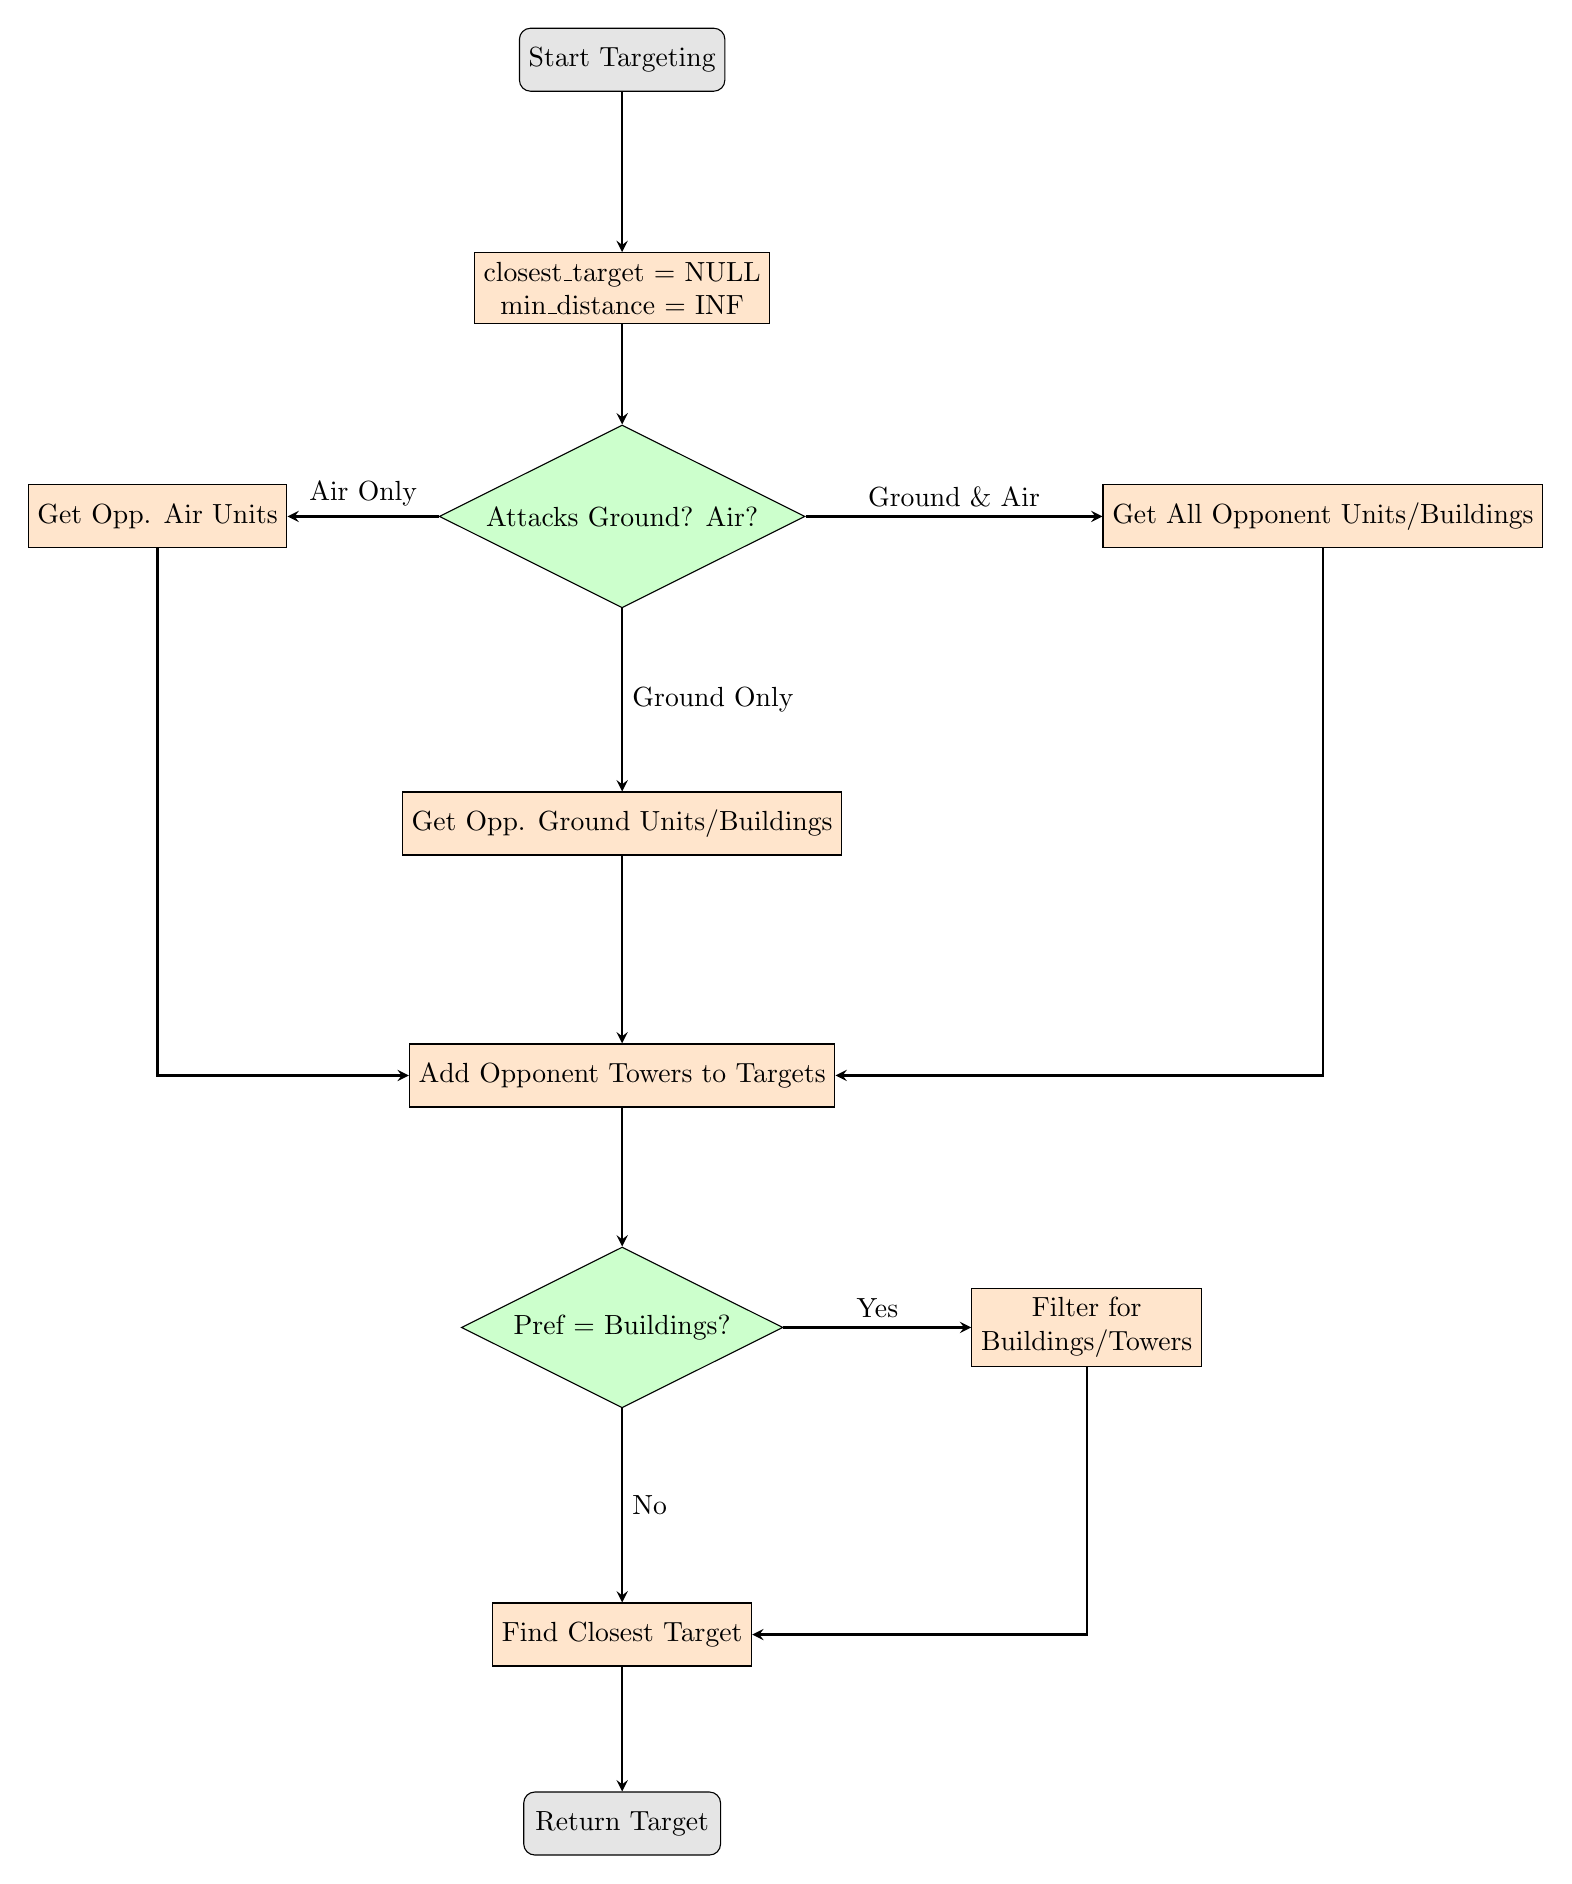
\begin{tikzpicture}[node distance=2.4cm]
\node (start) [startstop] {Start Targeting};
\node (initVar) [process, below of=start, yshift=-0.5cm,align=center] {closest\_target = NULL \\ min\_distance = INF};
\node (attType) [decision, below of=initVar, yshift=-0.5cm] {Attacks Ground? Air?};
\node (getAll) [process, right of=attType, xshift=6.5cm] {Get All Opponent Units/Buildings};
\node (getGround) [process, below of=attType, yshift=-1.5cm] {Get Opp. Ground Units/Buildings};
\node (getAir) [process, left of=attType, xshift=-3.5cm] {Get Opp. Air Units};
\node (addTowers) [process, below of=getGround, yshift=-0.8cm] {Add Opponent Towers to Targets};
\node (pref) [decision, below of=addTowers, yshift=-0.8cm] {Pref = Buildings?};
\node (filterBld) [process, right of=pref, xshift=3.5cm,align=center] {Filter for \\ Buildings/Towers};
\node (loopTargets) [process, below of=pref, yshift=-1.5cm] {Find Closest Target};
\node (end) [startstop, below of=loopTargets] {Return Target};

\draw [arrow] (start) -- (initVar);
\draw [arrow] (initVar) -- (attType);
\draw [arrow] (attType) -- node[anchor=south] {Ground \& Air} (getAll);
\draw [arrow] (attType) -- node[anchor=west] {Ground Only} (getGround);
\draw [arrow] (attType) -- node[anchor=south] {Air Only} (getAir);
\draw [arrow] (getAir) |- (addTowers);
\draw [arrow] (getGround) -- (addTowers);
\draw [arrow] (getAll) |- (addTowers);
\draw [arrow] (addTowers) -- (pref);
\draw [arrow] (pref) -- node[anchor=south] {Yes} (filterBld);
\draw [arrow] (filterBld) |- (loopTargets);
\draw [arrow] (pref) -- node[anchor=west] {No} (loopTargets);
\draw [arrow] (loopTargets) -- (end);
\end{tikzpicture}%
}
\caption{Target Selection Flowchart}
\end{figure}

\FloatBarrier

\subsubsection{Chest Reward System Flowchart}
\begin{figure}[H]
\centering
\adjustbox{max height=0.8\textheight}{%
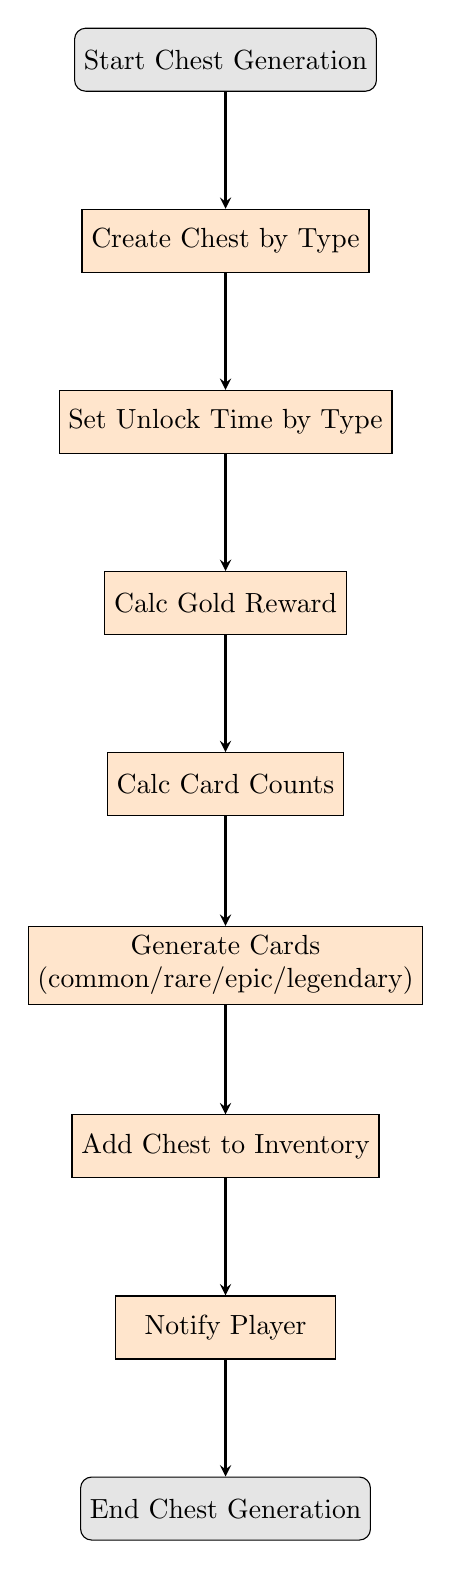
\begin{tikzpicture}[node distance=2.3cm]
\node (start) [startstop] {Start Chest Generation};
\node (createC) [process, below of=start] {Create Chest by Type};
\node (setTime) [process, below of=createC] {Set Unlock Time by Type};
\node (gold) [process, below of=setTime] {Calc Gold Reward};
\node (cards) [process, below of=gold] {Calc Card Counts};
\node (generate) [process, below of=cards, align=center] {Generate Cards \\ (common/rare/epic/legendary)};
\node (addChest) [process, below of=generate] {Add Chest to Inventory};
\node (notify) [process, below of=addChest] {Notify Player};
\node (end) [startstop, below of=notify] {End Chest Generation};

\draw [arrow] (start) -- (createC);
\draw [arrow] (createC) -- (setTime);
\draw [arrow] (setTime) -- (gold);
\draw [arrow] (gold) -- (cards);
\draw [arrow] (cards) -- (generate);
\draw [arrow] (generate) -- (addChest);
\draw [arrow] (addChest) -- (notify);
\draw [arrow] (notify) -- (end);
\end{tikzpicture}%
}
\caption{Chest Reward System Flowchart}
\end{figure}

\FloatBarrier

%----------------------------------------------------------------------------------
% TRACE TABLES
%----------------------------------------------------------------------------------
\section{Trace Tables}

%===============================
% MAIN SERVER LOOP TRACE TABLES
%===============================
\subsection{Main Server Loop Trace Tables}

\subsubsection{Scenario 1: Simple Two-Player Match}
\begin{table}[H]
\centering
\footnotesize
% Adjust columns to avoid overflow
\begin{tabularx}{\textwidth}{|c|p{3.5cm}|X|p{2.5cm}|p{2.5cm}|}
\hline
\textbf{Step} & \textbf{Condition} & \textbf{Action} & \textbf{player\_pool} & \textbf{active\_games}\\
\hline
1 & new\_connection=PlayerA & Create PlayerA & [PlayerA] & []\\
\hline
2 & matchmaking(PlayerA) & Add PlayerA to queue & [PlayerA] & []\\
\hline
3 & new\_connection=PlayerB & Create PlayerB & [PlayerA, PlayerB] & []\\
\hline
4 & matchmaking(PlayerB) & Add PlayerB to queue & [PlayerA, PlayerB] & []\\
\hline
5 & queue.count=2 & Create Game1 & [PlayerA, PlayerB] & [Game1]\\
\hline
6 & updateGames & UpdateGame(Game1) & [PlayerA, PlayerB] & [Game1]\\
\hline
\end{tabularx}
\caption{Main Server Loop Trace Table - Scenario 1}
\end{table}

\begin{table}[H]
\centering
\footnotesize
\begin{tabularx}{\textwidth}{|c|p{3.5cm}|X|p{2.5cm}|p{2.5cm}|}
\hline
\textbf{Step} & \textbf{Condition} & \textbf{Action} & \textbf{player\_pool} & \textbf{active\_games}\\
\hline
1 & new\_connection=PlayerC & Create PlayerC & [PlayerC] & []\\
\hline
2 & new\_connection=PlayerD & Create PlayerD & [PlayerC, PlayerD] & []\\
\hline
3 & no\_matchmaking & - & [PlayerC, PlayerD] & []\\
\hline
4 & PlayerC match request & Add to queue & [PlayerC, PlayerD] & []\\
\hline
5 & PlayerD match request & Add to queue & [PlayerC, PlayerD] & []\\
\hline
6 & queue.count=2 & Create Game2 & [PlayerC, PlayerD] & [Game2]\\
\hline
7 & updateGames & UpdateGame(Game2) & [PlayerC, PlayerD] & [Game2]\\
\hline
\end{tabularx}
\caption{Main Server Loop Trace Table - Scenario 2 (More Steps)}
\end{table}

\FloatBarrier

%===============================
% CARD DEPLOYMENT TRACE TABLES
%===============================
\subsection{Card Deployment Trace Tables}

\subsubsection{Scenario 1: Enough Elixir}
\begin{table}[H]
\centering
\footnotesize
\begin{tabularx}{\textwidth}{|c|p{2.2cm}|p{2.2cm}|X|X|}
\hline
\textbf{Step} & \textbf{Input} & \textbf{Check/Action} & \textbf{Outcome} & \textbf{New State}\\
\hline
1 & card\_id=101, pos=(3,4) & Check Valid Pos & Valid position & - \\
\hline
2 & Check card in hand & card 101? = True & OK & - \\
\hline
3 & Elixir=6, cost=4 & Enough elixir & Deploy possible & newElixir=2 \\
\hline
4 & Remove card from hand & Next card in deck & Cards in hand updated & hand=[102,103] \\
\hline
5 & Create Troop & type=TROOP & Troop placed & unitList += 1 \\
\hline
6 & Broadcast & - & Both see new troop & - \\
\hline
\end{tabularx}
\caption{Card Deployment - Scenario 1}
\end{table}

\subsubsection{Scenario 2: Insufficient Elixir}
\begin{table}[H]
\centering
\footnotesize
\begin{tabularx}{\textwidth}{|c|p{2.2cm}|p{2.2cm}|X|X|}
\hline
\textbf{Step} & \textbf{Input} & \textbf{Check/Action} & \textbf{Outcome} & \textbf{New State}\\
\hline
1 & card\_id=202, pos=(5,2) & Check Valid Pos & Valid position & - \\
\hline
2 & Card 202 in hand? & True & OK & - \\
\hline
3 & Elixir=2, cost=5 & Not enough & Return error & Elixir=2 (unchanged) \\
\hline
4 & Broadcast error & "Insufficient elixir" & - & - \\
\hline
\end{tabularx}
\caption{Card Deployment - Scenario 2}
\end{table}

\FloatBarrier

%===============================
% BATTLE UPDATE LOGIC TRACE TABLES
%===============================
\subsection{Battle Update Logic Trace Tables}

\subsubsection{Scenario 1: Regular Tick}
\begin{table}[H]
\centering
\footnotesize
\begin{tabularx}{\textwidth}{|c|p{2cm}|X|p{3cm}|X|}
\hline
\textbf{Step} & \textbf{Condition} & \textbf{Action} & \textbf{Result} & \textbf{Notes}\\
\hline
1 & time=50s $<$ max\_time=180 & Not in overtime & - & - \\
\hline
2 & Elixir regen=1 & p1Elixir=5$\rightarrow$6, p2Elixir=4$\rightarrow$5 & - & - \\
\hline
3 & UnitA health=20 $>$ 0 & Finds target & Moves or attacks & UnitB in range? \\
\hline
4 & Building1 health=100 & lifetime=10s & Attacks or pass & building1.lifetime=9.8 \\
\hline
5 & Tower check & HP $>$ 0 & No removal & - \\
\hline
6 & Broadcast state & - & Game states updated & - \\
\hline
\end{tabularx}
\caption{Battle Update Logic - Scenario 1}
\end{table}

\subsubsection{Scenario 2: Overtime Trigger}
\begin{table}[H]
\centering
\footnotesize
\begin{tabularx}{\textwidth}{|c|p{2cm}|X|p{3cm}|X|}
\hline
\textbf{Step} & \textbf{Condition} & \textbf{Action} & \textbf{Result} & \textbf{Notes}\\
\hline
1 & time=179.5s & next tick $\Rightarrow$ 180 & Check crowns & p1=1, p2=1 $\Rightarrow$ tie \\
\hline
2 & Overtime=flag & Overtime start & new end=240s & \\
\hline
3 & time=181s, OT active & Elixir regen $\times$2 & p1Elixir=7$\rightarrow$9 & - \\
\hline
4 & Attack tower & Tower HP=0 $\Rightarrow$ p1\_crowns=2 & - & p2 tower destroyed \\
\hline
5 & p1\_crowns $>$ p2\_crowns & game finished & broadcast result & p1=winner \\
\hline
\end{tabularx}
\caption{Battle Update Logic - Scenario 2}
\end{table}

\FloatBarrier

%===============================
% TARGET SELECTION TRACE TABLES
%===============================
\subsection{Target Selection Algorithm Trace Tables}

\subsubsection{Scenario 1: Melee Troop Prefers Buildings}
\begin{table}[H]
\centering
\footnotesize
\begin{tabularx}{\textwidth}{|c|p{3cm}|X|p{3cm}|c|}
\hline
\textbf{Step} & \textbf{Attacker Info} & \textbf{Action} & \textbf{Targets} & \textbf{Chosen}\\
\hline
1 & groundOnly=true, preference="BUILDINGS" & gather ground units & [UnitA(air), Bldg1, Tower1] & - \\
\hline
  2 & - & filter for buildings & [Bldg1, Tower1] & - \\
\hline
  3 & - & dist(Bldg1)=4, dist(Tower1)=10, closest = Bldg1 & [Bldg1] & Bldg1 \\
\hline
\end{tabularx}
\caption{Target Selection - Scenario 1}
\end{table}

\subsubsection{Scenario 2: Ranged Unit Attacks Ground \& Air}
\begin{table}[H]
\centering
\footnotesize
\begin{tabularx}{\textwidth}{|c|p{3cm}|X|p{3cm}|c|}
\hline
\textbf{Step} & \textbf{Attacker Info} & \textbf{Action} & \textbf{Potential Targets} & \textbf{closest\_target}\\
\hline
1 & groundAir=true & gather all Opp units & [UnitA, UnitB(air), Tower] & - \\
\hline
2 & preference="ANY" & no filter & [UnitA, UnitB, Tower] & - \\
\hline
  3 & distances=(UnitA=5, UnitB=4, Twr=8) & min=4 $\Rightarrow$ UnitB & [UnitB] & UnitB \\
\hline
\end{tabularx}
\caption{Target Selection - Scenario 2}
\end{table}

\FloatBarrier

%===============================
% CHEST REWARD TRACE TABLES
%===============================
\subsection{Chest Reward System Trace Tables}

\subsubsection{Scenario 1: Gold Chest}
\begin{table}[H]
\centering
\footnotesize
  \begin{tabularx}{\textwidth}{|c|p{5.0cm}|p{4cm}|p{2.5cm}|X|}
\hline
\textbf{Step} & \textbf{Input} & \textbf{Action} & \textbf{Value} & \textbf{Result}\\
\hline
1 & chest\_type="GOLD" & Create chest & - & chest \\
\hline
2 & set unlock time & 8 hours & chest.unlock=8h & - \\
\hline
3 & gold=calcReward(arena=3) & 120 & chest.gold=120 & - \\
\hline
4 & card counts & (common=12, rare=3) & - & total=15 cards \\
\hline
5 & generate cards & random from arena 3 pool & chest.cards=15 & - \\
\hline
6 & add chest to player & - & - & inventory +1 \\
\hline
7 & notify & SEND\_CHEST\_RECEIVED & - & - \\
\hline
\end{tabularx}
\caption{Chest Reward - Scenario 1}
\end{table}

\subsubsection{Scenario 2: Magical Chest}
\begin{table}[H]
\centering
\footnotesize
\begin{tabularx}{\textwidth}{|c|p{5.0cm}|X|p{2.5cm}|X|}
\hline
\textbf{Step} & \textbf{Input} & \textbf{Action} & \textbf{Value} & \textbf{Result}\\
\hline
1 & chest\_type="MAGICAL" & Create chest & - & chest \\
\hline
2 & unlock time=12h & chest.unlock=12h & - & - \\
\hline
3 & gold=calcReward(arena=5) & 400 & chest.gold=400 & - \\
\hline
4 & card counts & common=20, rare=8, epic=2 & - & total=30 \\
\hline
5 & generate cards & random from arena 5 pool & chest.cards=30 & includes epics \\
\hline
6 & add chest & player inventory & - & +1 chest \\
\hline
7 & notify & chest info $\Rightarrow$ user & - & - \\
\hline
\end{tabularx}
\caption{Chest Reward - Scenario 2}
\end{table}

\FloatBarrier

\end{document}
